%%%%%%%%%%%%%%%%%%%%%%%%%%%%%%%%%%%%%%%%%%%%%%%%%%%%%%%%%%%%%%%%%%%%
%% I, the copyright holder of this work, release this work into the
%% public domain. This applies worldwide. In some countries this may
%% not be legally possible; if so: I grant anyone the right to use
%% this work for any purpose, without any conditions, unless such
%% conditions are required by law.
%%%%%%%%%%%%%%%%%%%%%%%%%%%%%%%%%%%%%%%%%%%%%%%%%%%%%%%%%%%%%%%%%%%%

\documentclass[
  digital, %% This option enables the default options for the
           %% digital version of a document. Replace with `printed`
           %% to enable the default options for the printed version
           %% of a document.
  table,   %% Causes the coloring of tables. Replace with `notable`
           %% to restore plain tables.
  lof,     %% Prints the List of Figures. Replace with `nolof` to
           %% hide the List of Figures.
  lot,     %% Prints the List of Tables. Replace with `nolot` to
           %% hide the List of Tables.
  monochrome
  %% More options are listed in the user guide at
  %% <http://mirrors.ctan.org/macros/latex/contrib/fithesis/guide/mu/fi.pdf>.
]{fithesis3}
%% The following section sets up the locales used in the thesis.
\usepackage[resetfonts]{cmap} %% We need to load the T2A font encoding
\usepackage[T1,T2A]{fontenc}  %% to use the Cyrillic fonts with Russian texts.
\usepackage[
  main=slovak, %% By using `czech` or `slovak` as the main locale
                %% instead of `english`, you can typeset the thesis
                %% in either Czech or Slovak, respectively.
  english %% The additional keys allow
]{babel}        %% foreign texts to be typeset as follows:
%%
%%   \begin{otherlanguage}{german}  ... \end{otherlanguage}
%%   \begin{otherlanguage}{russian} ... \end{otherlanguage}
%%   \begin{otherlanguage}{czech}   ... \end{otherlanguage}
%%   \begin{otherlanguage}{slovak}  ... \end{otherlanguage}
%%
%% For non-Latin scripts, it may be necessary to load additional
%% fonts:
\usepackage{paratype}
\def\textrussian#1{{\usefont{T2A}{PTSerif-TLF}{m}{rm}#1}}
%%
%% The following section sets up the metadata of the thesis.
\thesissetup{
    date          = \the\year/\the\month/\the\day,
    university    = mu,
    faculty       = fi,
    type          = mgr,
    author        = Tomáš Márton,
    gender        = m,
    advisor       = RNDr. Daniel Tovarňák,
    title         = {Interaktivní správa a odhalování parsovacích pravidel pro logovací data},
    TeXtitle      = {Interaktivní správa a odhalování parsovacích pravidel pro logovací data},
    keywords      = {Logovanie, Clustering, Frequent Pattern Mining, Extended Nagappan-Vouk},
    TeXkeywords   = {Logovanie, Clustering, Frequent Pattern Mining, Extended Nagappan-Vouk},
    bib           = ./thesis.bib,
}
\thesislong{abstract}{
    Diplomová práca sa zaoberá odhaľovaním parsovacích vzorov systémových logov, konkrétne algoritmom Extended Nagappan-Vouk. Tento algoritmus vyhodnocuje a implementuje webové užíveteľské rozhranie pre tento algoritmus.
}
\thesislong{thanks}{
Rád by som poďakoval RNDr. Danielovi Tovarňakovi, vedúcemu tejto diplomovej práce za vedenie a podnetné návrhy. Ďalej by som sa rád poďakoval svojej rodine a priateľom za podporu pri písaní tejto práce.
}
\usepackage{makeidx}      %% The `makeidx` package contains
\makeindex                %% helper commands for index typesetting.
%% These additional packages are used within the document:
\usepackage{paralist} %% Compact list environments
\usepackage{amsmath}  %% Mathematics
\usepackage{amsthm}
\usepackage{amsfonts}
\usepackage{url}      %% Hyperlinks
\usepackage{multirow} %% table multirow
\usepackage{array} %% table cell vertical centering
\usepackage{tabularx}
\usepackage{listings}
\begin{document}

\chapter{Úvod}

Už od vynálezu počitačov produkuje každý softwér záznam o svojom behu. Tieto záznamy sa volajú logové súbory a slúžia programátorom a systémovým administrátorom na odladenie chýb programu a jeho monitorovanie. Logové súbory sú vytvárané programátormi vo forme viet hovorového jazyka, obsahujúcich všetky dôležité informácie o~udalosti v programe, ktorá práve nastala. Vo výsledku teda obsahujú jedinečné kvantum informácií, ktoré nie sú inak dostupné. Kvôli rozmachu technológií sa však rapídne zvýšil objem logovacích súborov, v ktorých už viac nie je možné triviálne nájsť požadované informácie. V praxi sa preto stretávame s prípadom, že síce máme data o udalostiach, ktoré nastali, ale nevieme ich nájsť a správne použiť, alebo ani nevieme, že tieto údaje máme. Sme teda bohatí na data, ale chudobní na informácie.
\par Z tohto dôvodu je nutné vedieť informácie o udalosti v programe z~logových súborov efektívne a automaticky extrahovať a predpripraviť na ďalšie spracovanie. To sa deje vytvorením parsovacích vzorov, ku~ktorým vieme každú udalosť jednoznačne priradiť. Momentálne však neexistuje nástroj, ktorý by takéto vzory vytvoril nad ľubovoľnou množinou vstupných logovacích súborov v dostatočnej kvalite. Existujúce algoritmy trpia na rôzne nedostatky, ako aj na potrebu detailného nastavenia vstupných parametrov.
\par V práci sa zaoberáme rozšírenou verziou algoritmu Nagappan-Vouk, vyvinutou vedúcim práce RNDr. Danielom Tovarňákom. Tento algoritmus slúži na odhaľovanie parsovacích vzorov v logovacích súboroch. Vychádza z algoritmov popísaných v práci, pričom odstra\-ňu\-je ich známe nedostatky za pridania jednoduchej užívateľskej interakcie. Cieľom tejto práce je teda naimplementovať užívateľské rozhranie, ktoré bude plne podporovať algoritmus Nagappan-Vouk, pokúsiť sa zlepšiť presnosť výsledných parsovacích vzorov a porovnať výsledky voči podobným algoritmom.
 \par Práca sa člení ....
\chapter{Problematika logovania}

Logové súbory sú neoddeliteľnou súčasťou každého softwéru. Či už sa jedná o operačný systém, aplikačný server, softwér v sieťových prvkoch alebo koncovú užívateľskú aplikáciu. 
\par Logové súbory zaznamenávajú všetky udalosti od štartu, cez beh a chybové stavy až po ukončenie aplikácie. Ich analýza je často jediným spôsobom, ako odhaliť chybu, lebo logovanie nijako nenarúša ani neovplyvňuje beh programu. To predstavuje presný opak analýzy bežiaceho programu, pri ktorej analytický proces priamo komunikuje s programom za časovo alebo zdrojovo kritických podmienok  \parencite{jvaldman}. Analýza logových súborov sa takisto môže využiť aj na detekciu anomálií, monitorovanie systému, odhadovanie a plánovanie záťaže systému \parencite{logengineering}.
\par Do logových súborov sú zapisované pološtrukturované správy, ktoré vývojári softwéru používajú kvôli jednoduchosti a flexibilite \parencite{he2016, ibm}. Informácie, ktoré sa zvyčajne nachádzajú v popise v každej logovacej správe \parencite{weblog, datapreprocessing, sshd}, sú:
\begin{itemize}
  \item dátum a čas
  \item ip adresa alebo hostname
  \item komponenta
  \item protokol
\end{itemize}
\par Vo všeobecnosti síce nie je ustálený jednotný formát správ, ale existujú dobre známe formáty ako napr. \emph{Common Log Format}, používaný pre logovanie http požiadavkov \parencite{CLF} , flexibilnejši \emph{Extended Log Format} \parencite{ELF} alebo \emph{Syslog format}, využívaný pre logovanie udalostí v systéme Unix \parencite{syslog}. Tieto formáty sú často využívané a existujú pre ne aj analytické nástroje. \

\section{Motivácia}

\par Hoci je zapisovanie a ukladanie logových súborov jednoduchá a lacná úloha, ich ďalšia analýza môže zabrať značné zdroje, čas aj sofistikované metódy. V extrémnych prípadoch môže jeden uzol vygenerovať až okolo pol milióna správ za deň, čo v sledovanom systéme vyústilo do 400 GB nekomprimovaných dát za 2 mesiace \parencite{google}. Aj keď sa odprostíme od takýchto prípadov, logovacie súbory sú stále príliš veľké na manuálne spracovanie, a preto je potrebné proces ich spracovania automatizovať. Počas tohto procesu extrahujeme z logovacej správy jej statickú a dynamickú časť. Statická časť predstavuje konštantný reťazec znakov a budeme ho ďalej nazývať parsovací vzor. Dynamickú časť tvoria parametre parsovacieho vzoru a môžu byť pre každú správu rôzne. Výsledok extrakcie môžeme vidieť v tabuľke \ref{tab:a}, kde je dynamická časť znázornená znakom \emph{*}. 

\begin{table}[htbp]
\centering
\begin{tabularx}{\textwidth}{X}
\multicolumn{1}{c}{Logové správy}                                                                 \\ \hline
Generating 768 bit RSA key                                     \\
Generating 2048 bit RSA key                                    \\
Illegal user admin from 218.49.183.17                          \\
Illegal user guest from 218.49.183.17                          \\
Failed password for test from 218.49.183.17 port 49266 ssh2    \\
Accepted password for test from 192.168.15.135 port 49266 ssh2 \\
Failed password for root from 218.49.183.17 port 1066 ssh2     \\
Accepted password for root from 192.168.20.185 port 1066 ssh2  \\
\multicolumn{1}{c}{\multirow{2}{*}{ $\Big\Downarrow$ }}                                                             \\
\multicolumn{1}{c}{}                                                                              \\
\multicolumn{1}{c}{Nájdené parsovacie vzory}                                                      \\ \hline
Generating * bit RSA key                                      \\
Illegal user * from *                                          \\
* password for * from * port * ssh2                           
\end{tabularx}
\caption{Logové správy z sshd a ich parsovacie vzory}
\label{tab:a}
\end{table}

\par Triviálny prístup je použiť jednoduchú sadu vzorov napísaných použitím regulárnych výrazov. Je to síce zlepšenie, ale bez špecifickej znalosti zdrojového kódu nie je možné odhaliť všetky vzory. Navyše sa ukázalo ako neudržateľné spravovať takéto vzory dlhodobo, kedže logovacie správy sa často menia \parencite{xu2010}. Preto je potrebné mať k dispozícií nástroj, ktorý vzory odhalí automaticky.









\chapter{Odhaľovanie parsovacích vzorov správ}

Odhaľovanie parsovacích vzorov sa z~rozšírením distibuovaných sytémov a cloudu a tým spojeného nárastu objemu logovacích správ stáva pomerne dobre študovaným problémom. Bolo vyvynutých mnoho algoritmov riešiacich daný problém, ale žiaden z~nich zatiaľ neponúka postačujúce riešenie. Medzi najčastejšie používané patria riešenia založené na analýze zdrojových kódov alebo na metóde clustrovania.

\section{Analýza zdrojových kódov}

Je to pomerne presná metóda, kde za pomoci statickej analýzy vieme vo väčšine prípadov odhaliť všetky parsovacie vzory.
Rôzne programovacie jazyky ale používajú rôzny štýl logovania. Programovací jazyk C napr. používa volanie funkcie \emph{printf}.
V~tomto prípade sa snažíme nájsť volania tejto funkcie a zároveň odvodiť typy parametrov.
Pre objektovo orientované jazyky je situácia trochu komplikovanejšia, ako môžeme vidieť na obr. \ref{fig:static}. Po~prvé, vo väčšine prípadov používajú nejakú logovaciu abstrakciu a jej rozhranie, ktoré musíme identifikovať. Po~druhé, v~objektovo orientovanom programovaní sa na výpis reprezentácie objektu používa metóda \emph{toString}, čo je aj dôvod, prečo sú nájdené parsovacie vzory neúplné a je nutné ďalej rekurzívne investigovať metódu \emph{toString} na všetkych parametroch nájdeného parsovacieho vzoru.

\begin{figure}[htbp]
\centering
\begin{minipage}{0.9\textwidth}
\lstset{tabsize=4,columns=flexible,breaklines=true,breakatwhitespace=true, showstringspaces=false}
\begin{lstlisting}
class Session {
	String uid;
	
	@Override
	public String toString() {
		return "session with uid=" + uid;
	}
}

if (logger.isDebugEnabled()) {
	logger.debug("Transport error in " + session);
}

2017-05-12 20:52:39 DEBUG SomeService:19 - Transport error in session with uid=92ebcb67fe33s
\end{lstlisting} 		
\end{minipage}
\caption{Logovacia správa a kód, ktorý ju spôsobil v~jazyku Java}
\label{fig:static} 
\end{figure}

Hlavným negatívom, ktorý vyplýva z~podstaty analýzy zdrojových kódov, je značné množstvo času potrebné na správne identifikovanie parsovacích vzorov. Túto analýzu musíme vykonať pre každú novú verziu zdrojových kódov, čo ďalej zvyšuje zložitosť. Podmienkou u~tejto metódy je aj potreba mať prístup k~zdrojovým kódom, čo nie je vždy možné. 

\section{ Metóda clustrovania}
Pre potreby definície clustrovania logovacích správ si zadefinujme logovaciu správu ako bod definovaný n-početnou množinou nominálnych atribútov. Potom clustrovanie vieme popísať ako hľadanie rozdelenia takýchto bodov do konečnej skupiny kategórií -- clustrov, kde body v~jednom clustri sú si navzájom podobné, a zároveň čo najviac rozdielne od členov iných clustrov na základe svojich atribútov \parencite{iplom}. Na určenie toho, ako veľmi sú dve správy podobné, sa používa vzdialenostná funkcia. Ako bolo spomenuté v \parencite{logcluster}, vzdialenostné funkcie tradičných clustrovacích algoritmov vyžadujú tieto vlastnosti: 

\begin{enumerate}
  \item tokeny prevažne numerického tvaru
  \item fixný a nízky počet tokenov
  \item možnosť ignorovať poradie
  \item atribúty prevažne numerického tvaru 
  \item fixný a nízky počet atribútov 
\end{enumerate}

Tieto vlastnosti ale body reprezentujúce logovacie správy nespĺňajú. Je to spôsobené tým, že body s nominálnymi atribútmi mávajú často variabilný počet atribútov. Preto nie je triviálne určiť, ako sa bude vzdialenosť týchto bodov merať, aj keď existujú vzdialenostné funkcie pre body s nominálnymi atribútmi, napr. Jaccardov koeficient \parencite{slct}. Ďalej v \parencite{logcluster} bolo ukázané, že doterajšie vzdialenostné funkcie nepracujú presne v pri počte atribútov vyššom ako 10 a často neodhalia cluster. Kombinácia týchto vlastností spôsobuje, že tradičné vzdialenostné funkcie sú na clustrovanie logovacích správ nevhodné. Spôsobov, podľa ktorých možno jednotlivé clustre vytvárať, je niekoľko a každý algoritmus používa svoj postup, ako si ukážeme ďalej. Najprv si ale pre nasledujúcu časť zadefinujeme pojmy, ktoré budeme používať pri popise algoritmov. Logovací súbor budeme nazývať dataset, jeho jednotlivé riadky budeme považovať za správy, ktorých každé slovo bude reprezentovať jeden token. Ďalej kvôli všeobecne zaužívanej konvencii budeme dynamickú časť nájdeného parsovacieho vzoru označovať ako wildcard a v~samotnom vzore ho budeme nahradzovať znakom \emph{*}. 


\subsection{SLCT - Simple Logfile Clustering Tool}
Tvorca SLCT \parencite{slct, slctloghound} si všíma 2 kľúčové vlastnosti logovacích súborov, o~ktoré sa opieral pri tvorbe algoritmu. Prvá vlastnosť je, že väčšina slov sa v~datasete nevyskytuje často a nezanedbateľná časť dokonca len raz. Druhá vlastnosť hovorí, že medzi slovami, ktoré sa vyskytujú často, je silná korelácia. Neformálne povedané, často sa vyskytujúce slová tvoria statickú časť a zvyšné slova dynamickú časť logovacej správy. Algoritmus na vstupe očakáva hraničnú hodnotu N, podľa ktorej určí, či bude dané slovo považované za statickú alebo dynamickú časť.  SLCT pracuje v~nasledujúcich troch krokoch.

\begin{enumerate}
  \item Všetky správy v~datasete rozloží na dvojice \emph{(pozícia, token)} a spočíta počet výskytov danej dvojice v~datasete. Pre rozklad správy na tokeny sa používa ako delimiter znak medzery. Ak výskyt dvojice prekračuje hraničnú hodnotu N, dvojicu nazývame frekventovaná. Napr. \emph{(1, Generating)}.
  \item Pre každú správu v~datasete vezme algoritmus všetky frekventované dvojice, ktoré potom spolu tvoria kandidátnu množinu, napr. \emph{{(1,Generating), (3,bit), (4,RSA), (5, key)}}. 
  \item Ak sa kandidátna množina nachádza v~logovacom súbore častejšie ako hraničná hodnota N, potom je zvolený cluster. Cluster je vytvorený doplnením wildcard za chýbajúce pozície v~riadku, takže vysledný pattern vyzerá takto \emph{Generating * bit RSA key}.
\end{enumerate}

Riadky, ktoré nepatria k~žiadnemu clustru, tvoria špeciálny cluster nazývaný outliers. Všimnime si, že algoritmus vôbec nezaznamenáva pozície medzier ani počet tokenov v~pôvodnej správe. Preto kvôli spôsobu, akým tvorí clustre, SLCT nevie odhaliť wildcard na konci riadku. Vezmime si kandidátnu množinu $\{(1,Illegal), (2,user), (4,from)\} $. SLCT vytvorí pattern \emph{Illegal user * from}. Správny pattern by mal vyzerať takto  \emph{Illegal user * from *}.

\subsection{Naggapan-Vouk algoritmus}
Kľúčová vlastnosť, na ktorej Naggapan a Vouk postavili ich algoritmus \parencite{nagappanvouk}, je skutočnosť, že keď sa konkrétny pattern nachádza v~datasete na viacerých miestach z~rôznymi parametrami, jeho statická časť sa bude vyskytovať vo väčšine prípadov, zatiaľ čo dynamická časť len pár krát. Preto Nagappan-Vouk buduje tabuľku frekvencií, ako vidíme v tab. \ref{fig:naggapan}. Priebeh algoritmu:

\begin{enumerate}
  \item Vybudujeme si frekvenčnú tabuľku, ktorá obsahuje informáciu, koľko krát sa dané slovo nachádza na konkrétnej pozícií v~datasete. Neformálne povedané, riadky sú tokeny a stĺpce sú pozície, na ktorých sa token nachádza.
  \item Pre každú správu si vo frekvenčnej tabuľke vyhľadáme frekvencie všetkých tokenov správy. Nájdeme frekvenciu, ktorá sa vyskytuje najčastejšie. V~prípade, že takýchto frekvencií je viac, použijeme nižšiu frekvenciu.
  \item Každý token, ktorý má frekvenciu vyššiu alebo rovnú ako frekvencia nájdená v~minulom kroku, je označený ako statická časť. Zvyšné slová sú analogicky dynamická časť.
\end{enumerate}

\begin{table}[htbp]
\centering
\begin{tabularx}{175px}{ | X | c | c | c | c | c | }
\hline
           & 1 & 2 & 3 & 4 & 5 \\ \hline
768        & 0 & 1 & 0 & 0 & 0 \\ \hline
2048       & 0 & 1 & 0 & 0 & 0 \\ \hline
bit        & 0 & 0 & 2 & 0 & 0 \\ \hline
Generating & 2 & 0 & 0 & 0 & 0 \\ \hline
key        & 0 & 0 & 0 & 0 & 2 \\ \hline
RSA        & 0 & 0 & 0 & 2 & 0 \\ \hline
\end{tabularx}
\caption{Frekvenčná tabuľka pre algoritmus Nagappan-Vouk}
\label{fig:naggapan}
\end{table}

Algoritmus Nagappan-Vouk odhalí aj wildcard na poslednej pozícií, ale generuje prekývajúce sa clustre a v~prípade málo frekventovaných správ neodhalí daný vzor. Algoritmus nepodporuje žiadnu formu vstupných parametrov, ktorá by zlepšila výsledky.

\subsection{IPLoM - Iterative partitioning log mining}
Algoritmus IPLoM \parencite{iplom}  funguje odlišne od algoritmov popísaných vyššie. Pracuje na princípe hierarchického rozdeľovania logových správ na segmenty, kde na konci algoritmu listy v~tejto hierarchickej štruktúre sú clustre, z~ktorých budú vytvorené parsovacie patterny. Algoritmus pracuje takto:

\begin{enumerate}
  \item Rozdelenie podľa počtu tokenov. Vychádza z~predpokladu, že každá správa, ktorá bola vygenerovaná rovnakým patternom, bude mať rovnakú dĺžku. Každý segment teda obsahuje n-tice, kde n je počet tokenov v~každej správe.
  \item Rozdelenie podľa pozície tokenu. Pre každý segment nájdeme pozíciu tokenu, na ktorej segment obsahuje najmenej unikátnych hodnôt naprieč všetkými správami. Segment ďalej rozdelíme podľa hodnôt na nájdenej pozícii.
  \item Rozdelenie podľa hľadania bijekcie. Pred samotným hľadaním bijekcie sú zo segmentu najskôr odčlenené správy, ktoré podľa heuristiky \emph{cluster goodness treshold} už formujú dobrý cluster. Pre zvyšné správy nájdeme 2 rôzne pozície tokenov, ktoré obsahujú najviac unikátnych hodnôt. Hľadáme bijekciu medzi množinami tokenov na týchto 2 pozíciách. Ak bijekcia existuje, správy sú odčlenené do novej časti. Ak miesto bijekcie existuje vzťah \emph{1-N} alebo \emph{N-1}, použijeme heuristiku \emph{lower and upper treshold}. V~prípade vzťahu \emph{N-M} sú buď ignorované alebo ďalej rozdelené na vzťahy \emph{1-N}.
  \item Formovanie clustrov. Každý finálny segment reprezentuje cluster. Pattern získame tak, že pozície tokenov s~kardinalitou unikátnych hodnôt rovnou 1 považujeme za statickú časť a zvyšné pozície za dynamickú časť patternu.
\end{enumerate}

IPLom bol navrhnutý tak, aby našiel všetky parsovacie vzory v~prvotnom behu bez nutnosti špecifikovať vstupné nastavenia. V~skutočnosti ale podporuje 4 nastavenia, ktorými môžme obmedziť počet nájdených vzorov ako aj ich granularitu \parencite{nagappanvouk}.

\subsection{Logcluster}

Logcluster je algoritmus, ktorý má vyriešiť známe nedostatky SLCT \parencite{logcluster}. Rovnako ako SLCT si všíma výskyt frekventovaných slov v~správach, ale na~rozdiel od SLCT neberie do úvahy ich pozíciu. Vďaka tomu vie algoritmus priradiť do jedného clustru aj správy, ktoré nemajú rovnaký počet tokenov. Logcluster vezme vstupný parameter \emph{s}  a rozdelí správy do clustrov tak, aby v~každom bolo aspoň \emph{s} správ. Ak je hodnota parametru \emph{s} určená zle, algoritmus produkuje buď príliš špecifické alebo príliš všeobecné parsovacie vzory. Autori preto dávajú odporúčanie, ako tento parameter správne nastaviť. Algoritmus podporuje prácu s~viacerými oddelovačmi slov, čo je v~praktickom použití veľmi potrebné a považujeme to za veľkú výhodu \parencite{logclustertool}. Pre ešte lepšie výsledky algoritmus používa heuristiky \emph{aggregate \, support} a \emph{join cluster}. Vysledné parsovacie vzory používajú pre wildcard zápis v~tvare \emph{*\{m,n\}}, napr. \emph{Generating *\{1,1\} bit RSA key}. Tento zápis označuje \emph{m} až \emph{n} tokenov oddelených delimitrom.


\subsection{Nedostatky}
Všetky vyššie zmienené algoritmy -- SLCT, Nagappan-Vouk a IPLoM, sú založené na pozícií tokenu v~správe. Z~toho vyplýva, že nie sú schopné detegovať dynamickú časť parsovacieho vzoru, ktorá by sa skladala z~viacerých tokenov. Ďalším nedostatkom týchto algoritmov je prekrývanie výsledných clustrov, ktoré by sa dalo odstrániť dodatočnou úpravou a spojením prekrývajúcich sa parsovacích vzorov. Logcluster tieto nedostatky síce nemá, ale správne nastavenie jeho heuristík môže byť náročná úloha.
\chapter{Rekurzívne clustrovanie pod dohľadom užívateľa}

Všetky algoritmy zmienené v~predchádzajúcej kapitole pomerne dobre odhaľujú parsovacie vzory, ktoré sa v~danom datasete objavujú často, a ich výsledky sú presné. Aby sme ale dosiahli odhalenie všetkých parsovacích vzorov pri zachovaní vysokej presnosti, musíme sa vysporiadať s~obmedzeniami clustrovacích algoritmov \parencite{Tovarnak2017}.

\subsection*{Rozdelenie správy na tokeny}
Prvým krokom všetkých prezentovaných algoritmov je rozdeliť parsovaciu správu na tokeny. V~tomto smere je potrebná väčšia variabilita pri~zadávaní oddeľovača slov. Nie všetky algoritmy totiž podporujú možnosť zadať aj iný oddeľovač ako medzera, ale ani podpora via\-cerých oddeľovačov tokenov nie je dostačujúca, ako si ukážeme na~príklade. \\

\indent \emph{Starting server with param timeout=2000 ms} \\
\indent \emph{Processing request 127.0.0.1/api/patterns?page-size=10\&page=3} \\

V~prvom prípade chceme použiť ako delimiter aj znak \emph{=} . V~druhom prípade je žiadúce, aby celá url adresa bola zachytená ako jeden para\-meter. Delimiter \emph{=} teda použiť nechceme, a preto by možnosť použiť iný delimiter pre rôzne logovacie správy pomohla ďalej spresniť výsledné parsovacie vzory.

\subsection*{Vstupné parametre}
Hodnota vstupných parametrov je vo vačšine prípadov jedným z~hlav\-ných faktorov, ktorý ovplyvňuje kvalitu výsledných parsovacích vzorov.
Pre~tieto hodnoty existujú odporúčania, ale najpresnejší výsledok získame až po manuálnej analýze datasetu, kde užívateľ po prezre\-tí správ datasetu spustí párkrát daný algoritmus a pokúsi sa nájsť parametre, pre ktoré budú výsledné parsovacie vzory čo najpresnej\-šie.

\subsection*{Kontrola výsledných parsovacích vzorov}
V~závislosti od vyššie zmienených nastavení dostaneme parsovacie vzory, ktoré buď zodpovedajú našej predstave, alebo nie. Komplikovanejšia situácia nasáva v~prípade, ak neexistuje všeobecné nastavenie algoritmu, ktoré by vrátilo všetky parsovacie vzory v~potrebnej kvalite. Tento problém sa dá obísť užívateľským rozdelením datasetu na menšie časti a na každú časť pustiť algoritmus s~vlastným nastavením. Toto je ale komplikované, zdĺhavé, náchylne k~chybám a~v~ne\-poslednom rade aj užívateľsky neprívetivé.

\section{RURC -- Recursive User-Reviewed Clustering}
\label{sec:rurc}
Z~hore uvedeného rozboru vyplýva, že ideálny algoritmus by mal zahŕňať určitý stupeň užívateľskej interakcie a mal by vedieť pracovať aj nad vybranou podmnožinou daného datasetu.
\par Vedúci práce, RNDr. Daniel Tovarňák, preto v~\parencite{Tovarnak2017} navrhol syste\-matický postup nazvaný \emph{Recursive User-Reviewed Clustering} znázornený na obr. \ref{fig:rurc}. Výsledkom je proces, pri ktorom užívateľ rekurzívne spúšťa algoritmus nad datasetom, pričom v~každom priebehu má možnosť potvrdiť finálne parsovacie vzory a odfiltrovať z~datasetu správy, ktoré k~nim patria.
\par Tento proces prebieha v~nasledujúcich krokoch:

\begin{enumerate}
  \item Odstránenie správ z~datasetu, ktoré prislúchajú k~už odhaleným parsovacím vzorom.
  \item Úvodný beh algoritmu s~defaultnými parametrami.
  \item Užívateľ rozhodne, ktoré parsovacie vzory sú akceptovateľné, a~tým zároveň z~datasetu odstráni príslušné správy.
  \item Užívateľ buď:
  	\begin{enumerate}
   		 \item spustí algoritmus nad celým datasetom so zmenenými parametrami a pokračuje od bodu 3.
   		 \item označí množinu vzorov, ktoré nie sú vhodné, spustí algoritmus nad podmnožinou datasetu, ktorá prislúcha k~vyb\-raným vzorom, a 				pokračuje od bodu 3.
   		 \item ukončí proces. Proces tiež končí, ak už neostali žiadne správy na spracovanie.
 	 \end{enumerate}
\end{enumerate}

\begin{figure}[htbp]
 \centering 
 \begin{minipage}{\linewidth}
 	\centering
 	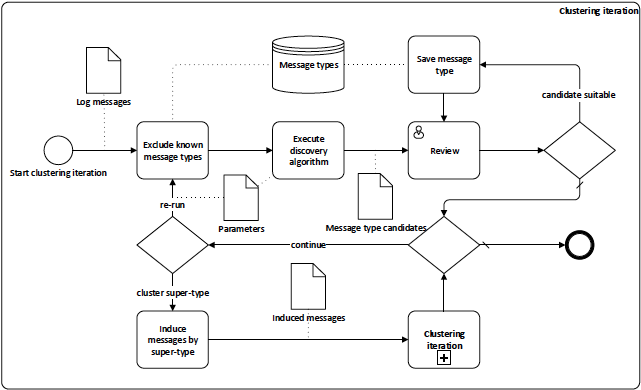
\includegraphics[width=\textwidth]{images/RURC.png} 	
 \end{minipage}
  \caption{Recursive User-Reviewed Clustering, obr. prevzaný z~\parencite{Tovarnak2017}}
  \label{fig:rurc}
\end{figure}


\section{Extended Nagappan-Vouk algoritmus}
\label{sec:eng}
RURC definuje všeobecné princípy analýzy logovacích súborov, avšak nešpecifikuje algoritmus, ktorý má byť použitý na clustrovanie správ.
Z~nedostatkov zmienených v~predchádzajúcej kapitole ale vyplýva, že žiaden algoritmus okrem LogCluster sa nehodí na použitie v~RURC.
\par RNDr. Daniel Tovarňák preto vyvinul algoritmus Extended Na\-gappan-Vouk určený pre použitie v~RURC, ktorý bude spĺnať všetky požiadavky RURC a zároveň bude jednoduchšie nastaviteľný ako LogCluster. Algoritmus produkuje parsovacie vzory vo formáte, ktorý popisuje parameter ako \emph{\%\{m,n\}} $\%\{m,n\}$. Podobne ako pri LogClustri to označuje \emph{m} až \emph{n} za sebou idúcich tokenov. Napr. parsovací vzor \emph{Software caused \%\{1,3\}} zachytí správu, ktorá obsahuje text \emph{Software caused} nasledovaný 1 až 3 slovami oddelenými medzerou. \newpage \par Postup algoritmu:

\begin{enumerate}
 \item Správy sa rozdelia na tokeny na základe užívateľom zadaných oddeľovačov slov.
 \item Algoritmus vybuduje frekvenčnú tabuľku rovnako ako pri klasickom Nagappan-Vouk algoritme. Rozdiel je však v~tom, že~algoritmus si ukladá aj pozície rozdeľovačov slov.
 \item Pre každú správu si vo frekvenčnej tabuľke vyhľadáme frekvencie všetkých tokenov správy. Rozdiel oproti Nagappan-Vouk algoritmu je ten, že hraničnú frekvenciu určíme metódou q-per\-centilu poďla užívateľom zadanej vstupnej hodnoty. Podľa toho označíme tokeny ako statickú časť alebo wildcard.
 \item Použitím heuristiky algoritmus skúsi odhaliť prekrývajúce sa clustre a v~prípade, že také clustre existujú, pripojí špecifickejší cluster k~viac všeobecnému.
 \item Algoritmus deteguje po sebe idúce sekvencie wildcard v~doposiaľ nájdených vzoroch a ak je to možné, tieto sekvencie spojí a~vytvorí
 vzor s~dolnou a hornou hranicou spojených tokenov.
\end{enumerate}

\subsection{Data mining}
\label{sec:data-mining}
Ako sme spomenuli v~sekcii \ref{sec:eng}, Extended Nagappan-Vouk produkuje parametre vzoru vo formáte \emph{\%\{m,n\}}. Výsledný parsovací vzor je teda kompaktný a užívateľsky čitateľný.  Tento formát vieme ďalej jednoduchou úpravou previesť na regulárny výraz používaný štandardnými knižnicami.
\par Po odhalení všetkých parsovacích vzorov väčšinou príde na rad data mining, tzn. pre každú logovaciu správu extrahujeme parametre jej parsovacieho vzoru. To vykonáme nájdením jej parsovacieho vzoru a vrátením zachytených skupín regulárneho výrazu. Triviálny, ale často používaný postup je iterovať cez všetky vzory až kým sa nenájde zhoda. V~najhoršom prípade to znamená prejsť celú množinu vzorov. Takýto prístup je ale neefektívny a môže spôsobovať výkonnostné problémy.
\par Kvôli odstráneniu vyššie zmienených problémov, RNDr. Daniel Tovarňák v~\parencite{regextrie} navrhol stromovú štruktúru Regex Trie - REtrie a~algoritmus, ktorý v~danej štuktúre nájde príslušný parsovací vzor so~zložitosťou $\mathcal{O}(t)$, kde $t$ je počet tokenov v~správe.
\par REtrie akceptuje parsovacie vzory vo formáte YAML súboru:

\begin{figure}[h]
\centering
\begin{minipage}{\textwidth}
\lstset{columns=flexible,breaklines=true,breakatwhitespace=true, showstringspaces=false}
\begin{lstlisting}
regexps:
  INT: [integer, '[0-9]+']
  STRING: [string, '[!-~]+']
  
patterns:
  default:
    pattern1:'Generating %{INT:var1} bit RSA key'
  ssh:
   pattern1:'Illegal user %{STRING:var1} from %{STRING:var2}'
\end{lstlisting} 		
\end{minipage} 
\end{figure}

Pod kľúčom regexps je zoradený zoznam typov regulárnych výrazov. Každý takýto typ sa skladá z~mena, dátového typu a samotného regulárneho výrazu. Kľúč patterns obsahuje parsovacie vzory, ktoré sú združené pod ľubovoľným identifikátorom skupiny vzorov. Parameter parsovacieho vzoru sa potom skladá z~odkazu na typ regulárneho výrazu a mena. Pri hľadaní vhodného typu sa postupuje zhora nadol a použije sa prvý vhodný typ, ktorý sa nájde. Preto je dôležité poradie, v~akom sú dané typy uvedené.  Aby sme mohli ťažiť z~tohto prístupu, výsledný systém musí vedieť zvládnuť konverziu medzi prezentovanými formátmi parsovacích vzorov.



 \printbibliography



\appendix %% Start the appendices.
\chapter{An appendix}
Here you can insert the appendices of your thesis.

\end{document}
